\documentclass[a4paper]{article}

\usepackage[czech]{babel}
\usepackage[utf8x]{inputenc}
\usepackage[T1]{fontenc}
\usepackage{amsmath}
\usepackage{graphicx}
\usepackage[left=2cm,text={17cm, 25.7cm},top=2cm]{geometry}

\title{\textbf{2. samostatná práce\\IMA\\Zadanie 9}}
\author{Adam Šulc - xsulca00\\ Tomáš Ulický - xulick01\\ Daniel Rudík - xrudik00\\ Ondrej Svoreň - xsvore01\\ Adrián Tomašov - xtomas32\\ Jozef Urbanovský - xurban66}
\date{}

\begin{document}
	\maketitle
	\begin{center}
		
\includegraphics[clip]{FIT.png}
	\end{center}
	\newpage
	\section*{1. príklad}
		1.  Riešenie\\	
		$t: f(x_0) + f'(x_0)(x - x_0)$ \\
		$n: f(x_0) - \dfrac{1} {f'(x_0)}(x - x_0)$\\
		\\
		\\
		$t: f(x_0) + f'(x_0)(x - x_0) = x_0^2-1+2x_0(x-x_0) = x_0^2-1+2x_0x-2x_0^2 = -x_0^2+2x_0x-1$ \\
		$n: f(x_0) - \dfrac{1} {f'(x_0)}(x - x_0) = x_0^2-1-\dfrac{1} {2x_0}(x-x_0) = x_0^2-1-\dfrac{x} {2x_0}+\dfrac{1}{2} = x_0^2 - \dfrac{1}{2x_0}x - \dfrac{1}{2}$\\
		\\
		\\	
		$
		\int_{0}^{x_0} 
		(x_0^2 - \dfrac{1}{2x_0}x - \dfrac{1}{2} - (-x_0^2+2x_0x-1)) dx =
		\int_{0}^{x_0} 
		(x_0^2 - \dfrac{1}{2x_0}x - \dfrac{1}{2} + x_0^2-2x_0x+1) dx =
		\int_{0}^{x_0} 
		(2x_0^2 - \dfrac{1}{2x_0}x -2x_0x+ \dfrac{1}{2} ) dx =
		2x_0^2\int_{0}^{x_0}1dx - \dfrac{1}{2x_0}\int_{0}^{x_0}xdx -2x_0\int_{0}^{x_0}xdx+ 	\dfrac{1}{2}\int_{0}^{x_0}1dx =
		\left[2x_0^2x - \dfrac{1}{2x_0}\dfrac{x^2}{2} - 2x_0\dfrac{x^2}{2} + \dfrac{1}{2}x\right]_0^{x_0} = \left(2x_0^3 - \dfrac{x_0^2}{4x_0} - \dfrac{2x_0^3}{2} + \dfrac{1}{2}x_0\right) - 0 =
		2x_0^3 - \dfrac{x_0}{4} - x_0^3 + \dfrac{1}{2}x_0 = x_0^3 - \dfrac{x_0}{4} + \dfrac{x_0}{2} = x_0^3 + \dfrac{1}{4}x_0
		$
		\\
		\\
		\\
		$x_0^3 + \dfrac{1}{4}x_0 = \dfrac{17}{2}$ \\
		$4x_0^3 +x_0 = 34$\\
		$x_0(4x_0^2+1) - 34 = 0$\\
		$2(4*2^2 + 1) -34 = 0$\\
		$x_0 = 2$\\
		\\
		2. Riešenie\\\\
		$t: f(x_0) + f'(x_0)(x - x_0)$ \\
		$n: f(x_0) - \dfrac{1} {f'(x_0)}(x - x_0)$\\
		\\
		\\
		$t: f(x_0) + f'(x_0)(x - x_0) = x_0^2-1+2x_0(x-x_0) = x_0^2-1+2x_0x-2x_0^2 = -x_0^2+2x_0x-1$ \\
		$n: f(x_0) - \dfrac{1} {f'(x_0)}(x - x_0) = x_0^2-1-\dfrac{1} {2x_0}(x-x_0) = x_0^2-1-\dfrac{x} {2x_0}+\dfrac{1}{2} = x_0^2 - \dfrac{1}{2x_0}x - \dfrac{1}{2}$\\
		\\
		\\	
		$
		\int_{-x_0}^{0} 
		(x_0^2 - \dfrac{1}{2x_0}x - \dfrac{1}{2} - (-x_0^2+2x_0x-1)) dx =
		\int_{-x_0}^{0} 
		(x_0^2 - \dfrac{1}{2x_0}x - \dfrac{1}{2} + x_0^2-2x_0x+1) dx =
		\int_{-x_0}^{0} 
		(2x_0^2 - \dfrac{1}{2x_0}x -2x_0x+ \dfrac{1}{2} ) dx =
		2x_0^2\int_{-x_0}^{0} 1dx - \dfrac{1}{2x_0}\int_{-x_0}^{0} xdx -2x_0\int_{-x_0}^{0}xdx+ 	\dfrac{1}{2}\int_{-x_0}^{0} 1dx =
		\left[2x_0^2x - \dfrac{1}{2x_0}\dfrac{x^2}{2} - 2x_0\dfrac{x^2}{2} + \dfrac{1}{2}x\right]_{-x_0}^0 = 0 - \left(2x_0^3 - \dfrac{x_0^2}{4x_0} - \dfrac{2x_0^3}{2} + \dfrac{1}{2}x_0\right) =
		-2x_0^3 + \dfrac{x_0}{4} + x_0^3 - \dfrac{1}{2}x_0 = -x_0^3 - \dfrac{1}{4}x_0
		$
	
	
		$-x_0^3 - \dfrac{1}{4}x_0 = \dfrac{17}{2}$ \\
		$-4x_0^3 -x_0 = 34$\\
		$-x_0(4x_0^2+1) - 34 = 0$\\
		$-(-2)(4*(-2)^2 + 1) -34 = 0$\\
		$x_0 = -2$\\
		\\
	
	\section*{2. príklad}
	
	$$\int_{0}^{\infty} \bigg( \frac{1}{(x+3)^2} - \frac{2}{x+3} - \frac{2}{x+1} + \frac{4x}{x^2+1} \bigg) dx$$
	$$\lim_{a\to\infty} \int_{0}^{a} \bigg( \frac{1}{(x+3)^2} - \frac{2}{x+3} - \frac{2}{x+1} + \frac{4x}{x^2+1} \bigg) dx$$
	$$\lim_{a\to\infty}  \bigg[- \frac{1}{x+3} -2ln|x+3| -2ln|x+1| +2ln|x^2+1| \bigg] ^a _{0}$$
	$$\lim_{a\to\infty}  \bigg[   ln \bigg| \frac{(x^2+1)^2}{(x+3)^2(x+1)^2}   \bigg|  - \frac{1}{x+3}  \bigg] ^a _{0}$$
	$$\lim_{a\to\infty}  \bigg[   ln \bigg( \frac{(x^2+1)}{(x+3)(x+1)}   \bigg)^2  - \frac{1}{x+3}  \bigg] ^a _{0}$$
	
	$$\lim_{a\to\infty}  \bigg[   ln \bigg( \frac{ 1 + \frac{1}{x^2} }{ 1+\frac{4}{x} + \frac{3}{x^2} }   \bigg)^2  - \frac{1}{x+3}  \bigg] ^a _{0}$$
	$$\bigg[ (ln1 + 0) - \bigg( ln\bigg(\frac{1}{9}\bigg)  + \frac{1}{3} \bigg)  \bigg] = \frac{1}{3} + 2ln(3)$$
	\newpage
	
	\section*{3. príklad}
	
	$$\int_{0}^{1} \frac{1}{x^5+32} dx= \frac{1}{32} \int_{0}^{1}\frac{1}{ 1+\frac{x^5}{2^5} } dx= \frac{1}{32} \int_{0}^{1} \frac{1}{ 1 - \big(\frac{-x}{2}\big)^5   }dx$$
	
	$$\frac{1}{32} \int_{0}^{1} \sum_{n=0}^{\infty} (-1)^n (\frac{x}{2})^{5n}dx$$
	$$\frac{1}{32}  \sum_{n=0}^{\infty} \int_{0}^{1}  (-1)^n (\frac{x}{2})^{5n}dx$$
	$$\frac{1}{32}  \sum_{n=0}^{\infty} \int_{0}^{1} \bigg( 1- \frac{x^5}{2^5}  + \frac{x^{10}}{x^{10}}  - \frac{x^{15}}{2^{15}} + ... + (-1)^n\bigg(\frac{x}{2}\bigg)^{5n} + ...  \bigg)dx$$
	
	$$ \frac{1}{32}  \bigg[ x - \frac{x^6}{6*2^5} + \frac{x^{11}}{11*2^{10}} - \frac{x^{16}}{16*2^{15}}  + ... +(-1)^n\frac{ x^{n+1} }{(x+1)2^{5n}} + ...\bigg]^{1}_{0} $$
	$$ \frac{1}{32} \frac{17212895}{17301504} \doteq \frac{0.9948853772}{32} \doteq 0.03109016803 $$
	\newpage
	
	\section*{4. príklad}
	
	$$f(x,y)=\frac{1}{1-4x^2-y^2}-\ln(x(4y^2-x^2-1))$$
	\\
	\begin{align*}
		1-4x^2-y^2 \neq 0\quad \wedge&\quad x(4y^2 - x^2 - 1) > 0 \\
		4x^2 + y^2 \neq 1\qquad &\quad (x > 0 \wedge 4y^2 - x^2 -1 > 0)\quad \vee&\ (x<0  \wedge 4y^2 - x^2 - 1 < 0)\\
		&\quad 4y^2 - x^2 > 1\ &\ 4y^2 - x^2 < 1
	\end{align*}
	
	\begin{figure}[h]
		\begin{center}
			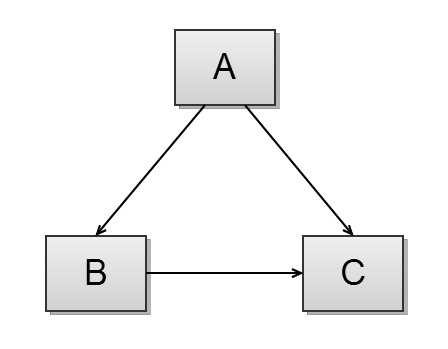
\includegraphics[scale=0.3]{graph.png}\\
		\end{center}
	\end{figure}
	
	\section*{5. príklad}
		\begin{align*}
			f(x,y) &= e^{3x+2y}(3x^2 - 6xy +8y^2)\\
			\\
			f'x &= 3e^{3x+2y}(3x^2 - 6xy +8y^2) + e^{3x+2y}(6x - 6y)\\
			f'y &= 2e^{3x+2y}(3x^2 - 6xy +8y^2) + e^{3x+2y}(-6x + 16y)\\
			\\
			e^{3x+2y}*3(3x^2 - 6xy +8y^2 + 2x - 2y) &= 0 /*2\\
			e^{3x+2y}*2(3x^2 - 6xy +8y^2 - 3x + 8y) &= 0 /*3\\
			\\
			5x - 10y &= 0\\
			5x &= 10y\\
			x &= 2y\\
			\\
			3(2y)^2 - 6(2y)*y + 8y^2 + 2(2y) - 2y &= 0\\
			12y^2 - 12y^2 + 8y^2 +4y - 2y &= 0\\
			8y^2 + 2y &= 0\\
			2y(4y+1) &= 0\\
			2y &= 0 \\
			y_1 &= 0 \\
			4y+1 &= 0\\
			4y &= - 1\\
			y_2 &= - \frac{1}{4}
		\end{align*}
		$$x_1 = 0\qquad x_2 = - \frac{1}{2}\\$$
		$$P_1\left[0;0\right]\qquad P_2\left[-\frac{1}{2};-\frac{1}{4}\right]\\$$
		\begin{align*}
			f''_{xx} &= 9e^{3x+2y}*(3x^2 - 6xy + 8y^2) + 6e^{3x+2y}\\
			f''_{xy} &= 6e^{3x+2y}*(3x^2 - 6xy + 8y^2) - 6e^{3x+2y}\\
			f''_{yy} &= 4e^{3x+2y}*(3x^2 - 6xy + 8y^2) + 16e^{3x+2y}\\
		\end{align*}
		Hessova matica:\\
		\begin{align*}
			\begin{vmatrix}
				f''xx & f''xy\\
				f''yx & f''yy\\
			\end{vmatrix}
			=
			\begin{vmatrix}
				6 & -6\\
				-6 & 16\\
			\end{vmatrix}
			= (6*16) - (-6)(-6) = 60 > 0
		\end{align*}
		V bode $P_1, P_2$ má lokálne minimum.\\
		\begin{align*}
			\begin{vmatrix}
				\frac{21}{2e^2} & - \frac{3}{e^2}\\
				-\frac{3}{e^2} & \frac{18}{e^2}\\
			\end{vmatrix}
			= \bigg(\frac{21}{2e^2}*\frac{18}{e^2}\bigg) - \bigg(\bigg(- \frac{3}{e^2}\bigg)\bigg(- \frac{3}{e^2}\bigg) = \frac{1}{e^4}\bigg(21*9 - 9\bigg) = \frac{180}{e^4} > 0\\
		\end{align*}
		\begin{align*}
			9e^{3(-\frac{1}{2})+2(-\frac{1}{4})}*
			\bigg(3\bigg(-\frac{1}{2}\bigg)^2 - 6\bigg(-\frac{1}{2}\bigg)-&\bigg(-\frac{1}{4}\bigg)+
			8\bigg(-\frac{1}{4}\bigg)^2\bigg) + 
			6e^{3(-\frac{1}{2})+2(-\frac{1}{4})} = \\ =
			9e^{-\frac{3}{2}-\frac{1}{2}}*\bigg(\frac{3}{4}-\frac{3}{4}+\frac{1}{2}\bigg) + 6e^{-2} =
			\frac{9}{e^2}&*\frac{1}{2}*\frac{6}{e^2} = 
			\frac{9}{2e^2}+\frac{6}{e^2} = \frac{9+12}{2e^2} = \frac{21}{2e^2}\\
			\\
			\frac{6}{e^2} * \frac{1}{2} - \frac{6}{e^2} = \frac{6}{2e^2} -& \frac{6}{e^2} =
			\frac{6 - 12}{2e^2} = -\frac{3}{e^2}\\
			\\
			\frac{4}{e^2} * \frac{1}{2} + \frac{16}{e^2} = \frac{4}{2e^2} +& \frac{16}{e^2} = \frac{4 + 32}{2e^2} = \frac{18}{e^2}
		\end{align*}
	
	
\end{document}